\chapter{Data reconstruction and selection}
\label{sec:Selection}
The data sample used in this analysis originates from \proton\proton collisions and has been recorded in the years 2011 at a center of mass energy $\sqs = 7 \tev$ and 2012 with $\sqs = 8 \tev$, corresponding to an integrated luminosity of \intlum{3 \invfb}.
This chapter describes and motivates the selection criteria for the reconstruction of the decays \LbToDpmunuX and \LbToLcmunu\footnote{If not stated otherwise, the $\mathcal{CP}$ conjugated decays \decay{\Lbbar}{\Dzb\antiproton\mup\neum} and \decay{\Lbbar}{\Lcbar\mup\neum} are included in those samples}.
As the \Dz and the \Lc are not stable enough to be directly indentified and detected, the subsequent decays \DToKpi and \LcTopKpi have been chosen for their reconstruction.
These decays leave a clear signature in the detector and can be well reconstructed at \lhcb, meaning that the pollution with background is small.
Furthermore, with this choice one ends up with the same final state particles for reconstruction in both signal and normalisation channel, namely \pKpi\mun.
Hence, any inefficiencies due to different interaction of particles with the detector should cancel, at least to first order.

One experimental difficulty arises due to the semileptonic nature of the signal and normalisation channel:
The neutrino cannot be reconstructed.
Consequently it is not possible to fully reconstruct the \Lb and to get a \Lb mass peak for the distinction between signal and background.
This leads to a high pollution of the data sample with backgrounds.

\section{Reconstruction of the decay \LbToDpmunuX}
The main strategy in the reconstruction process of the decay \LbToDpmunuX is to find events with the signature $\decay{X_{b}}{(\DToKpi) \mun \neumb X}$, where $X_b$ denotes a \bquark-quark containing hadron, first.
Then, the proton track is combined to the \Dz\mun vertex to make a \LbToDpmunuX candidate.
It is apparent that a main source of background will be a \decay{\Bd/\Bp}{\Dz\mun\neumb X} decay, where a random proton is added.
To better understand the selection criteria and the way this \textsc{combinatorial background} is reduced, it might be helpful to have a look at a sketch of a typical \LbToDpmunuX decay in Figure \ref{fig:DecaySketch} left.
\begin{figure}[tb]
	\centering
	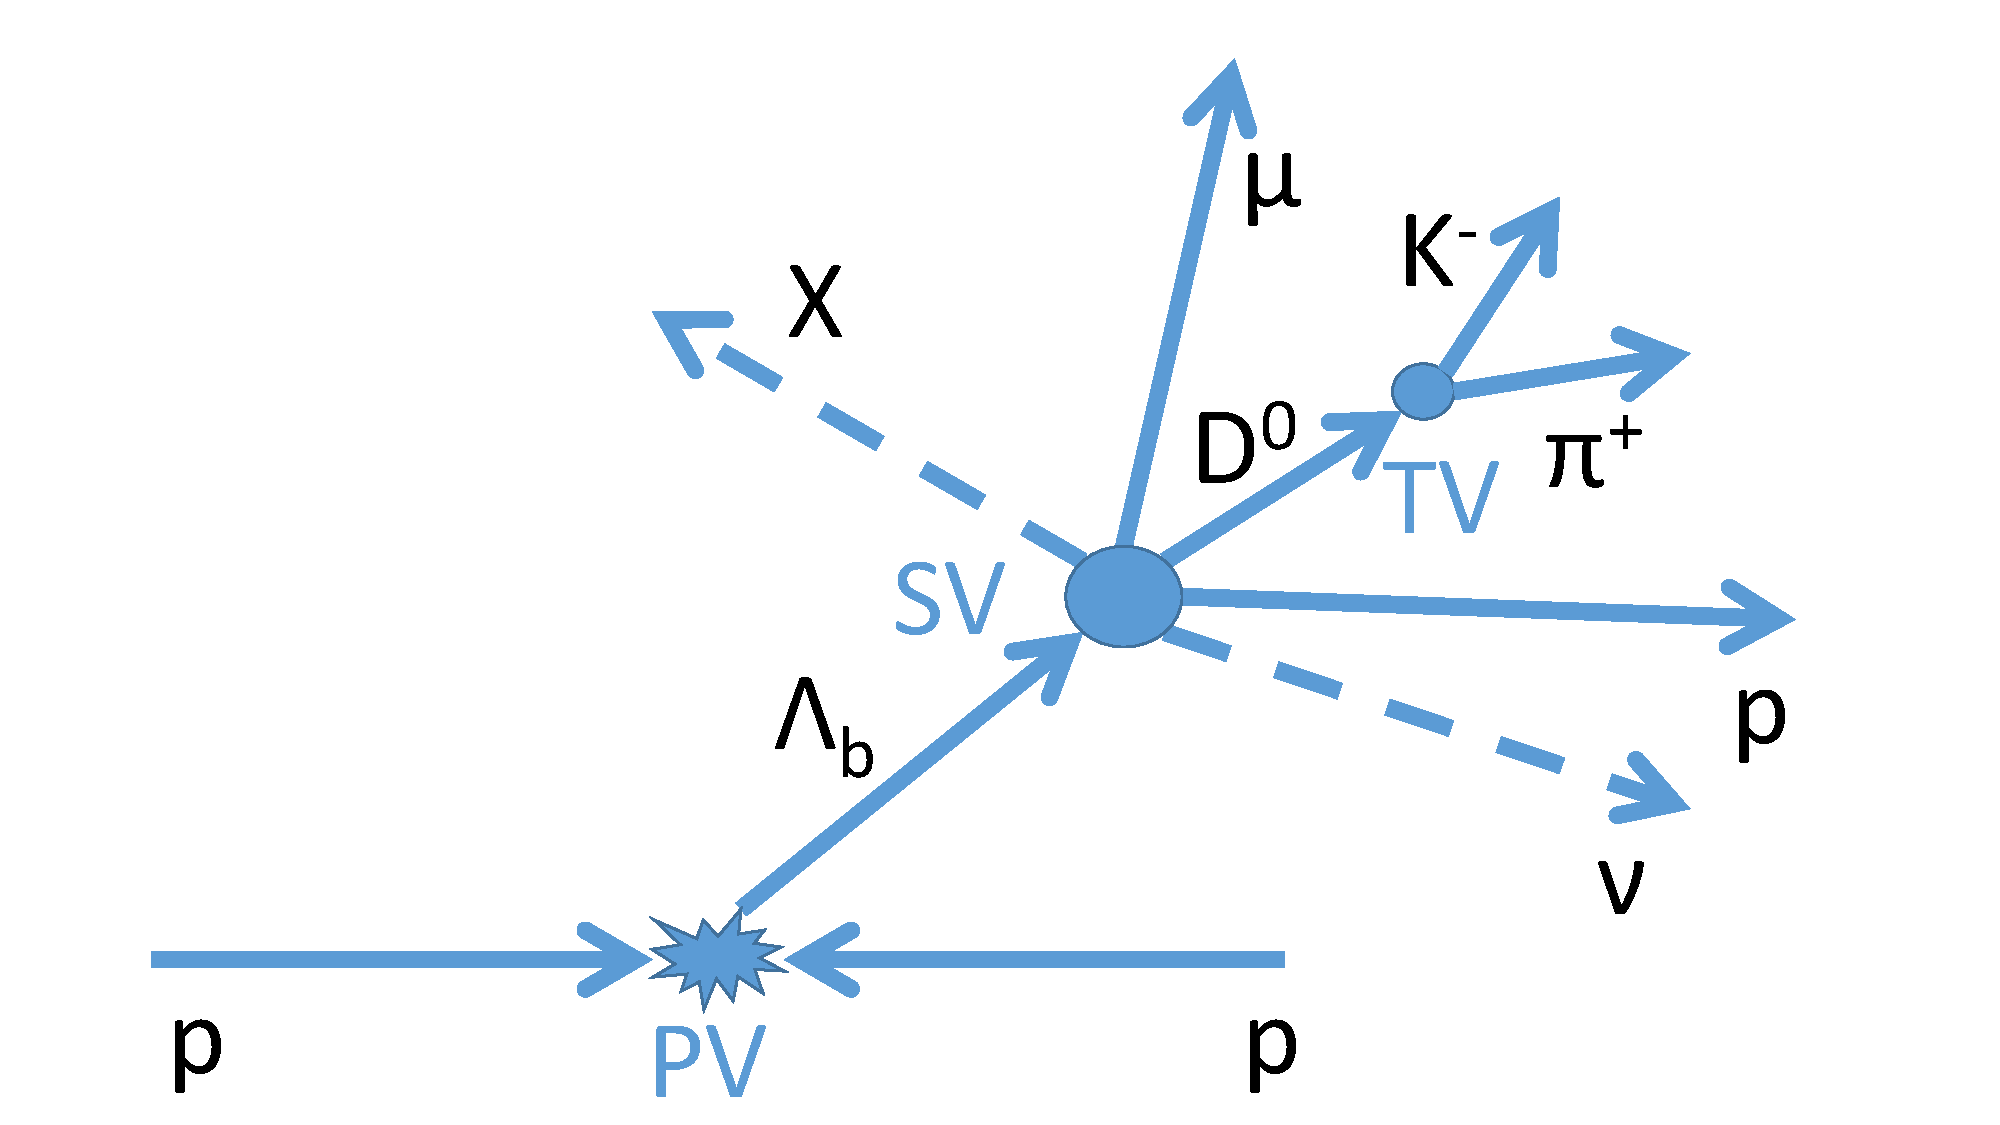
\includegraphics[width=0.49\textwidth]{decay_sketch_signal}
	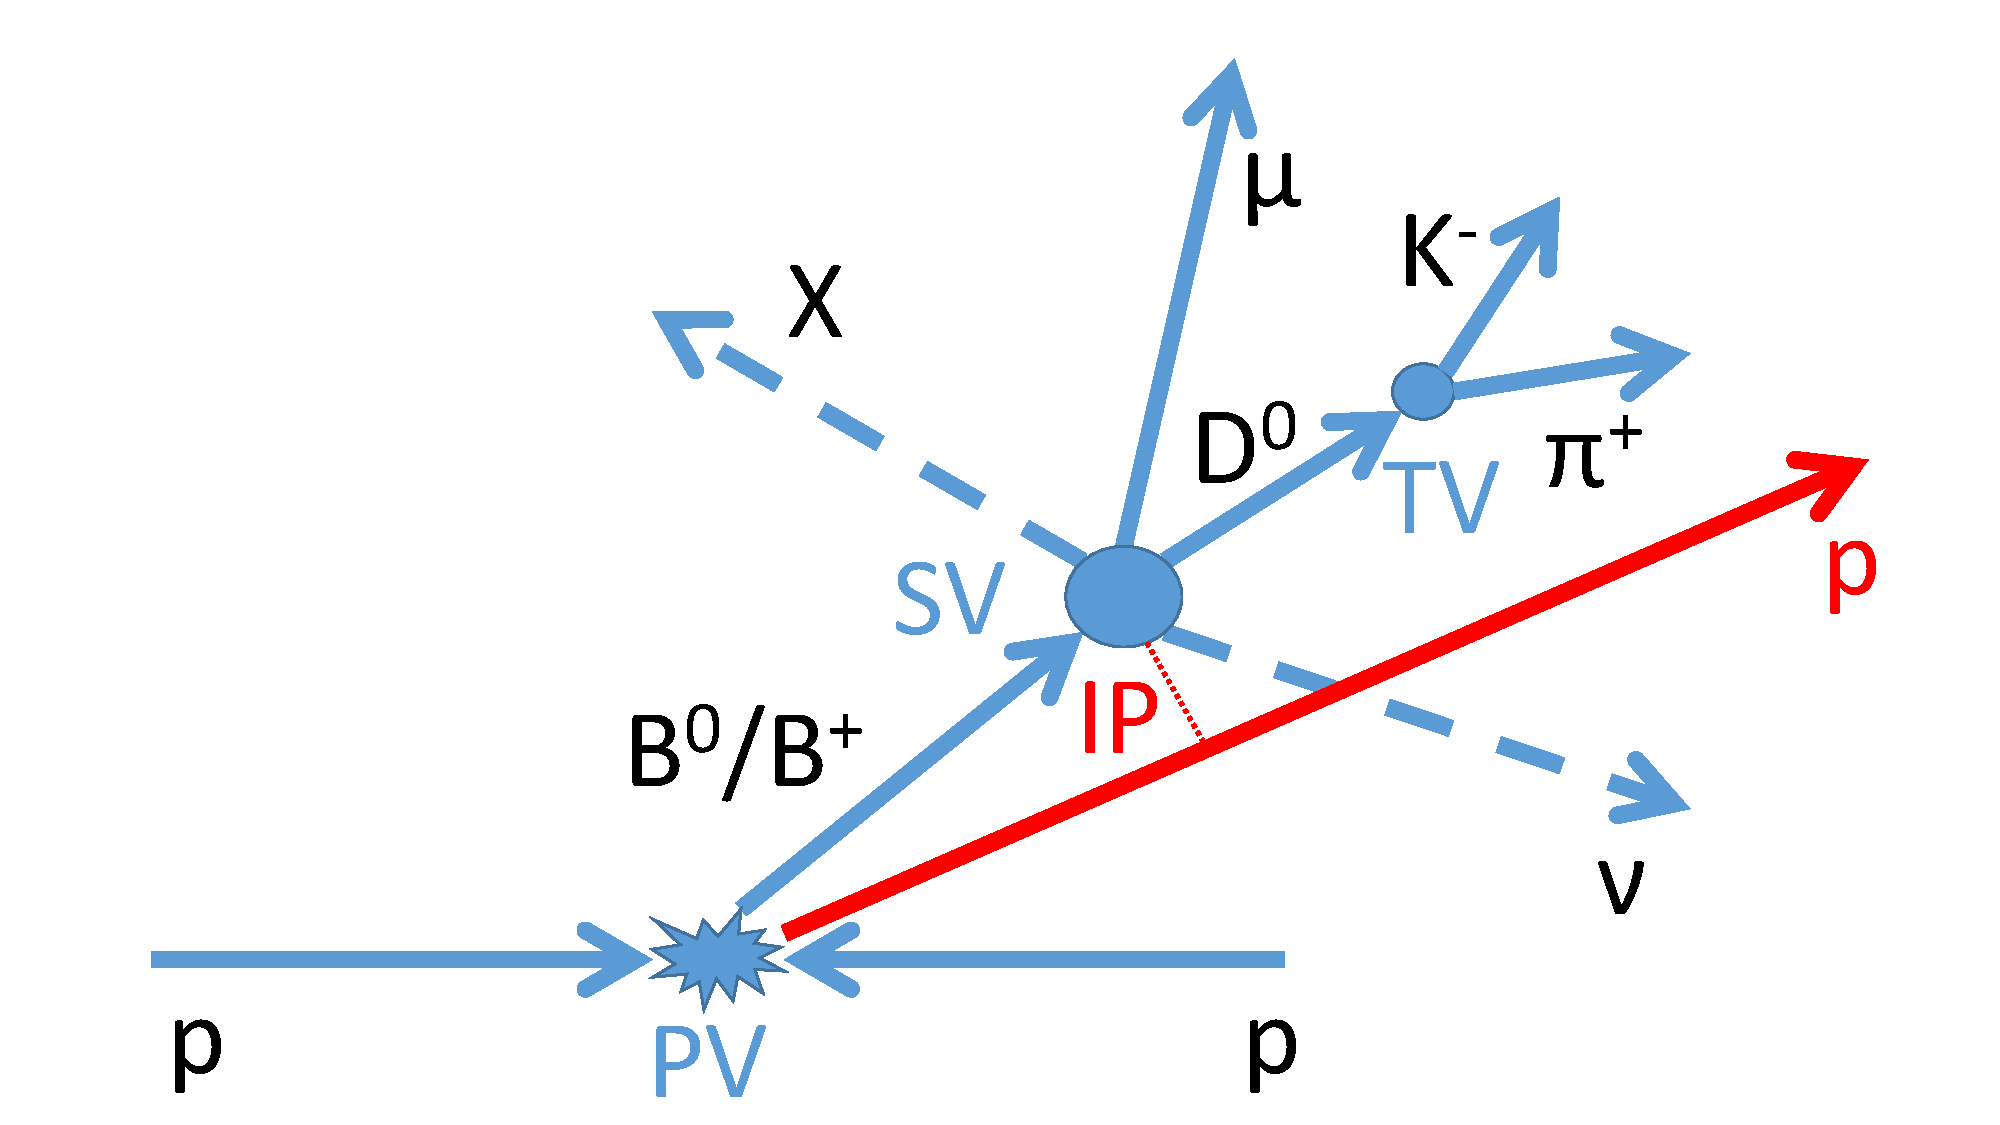
\includegraphics[width=0.49\textwidth]{decay_sketch_background}
	\caption{
        Sketch of the decay topology for a typical \LbToDpmunuX decay (left) and for the background decay \decay{\Bd/\Bp}{\Dz\mun\neumb X} with a randomly combined proton (right).
        In these background events the proton rather poorly makes a vertex with the \Dz\mun candidate, indicated by a large impact parameter (IP).
        Particle tracks drawn with a dashed line are not reconstructed.
        This sketch does neither account for the correct distances between the vertices nor the boost of the particles in $z$-direction.
    }
	\label{fig:DecaySketch}
\end{figure}
Due to its relatively long lifetime, it is typical for a \Lb or in general a \bquark-hadron that it decays at a so called \textsc{secondary vertex (SV)} displaced from the primary \proton\proton interaction, the \textsc{primary vertex (PV)}.
The decay products \Dz, \mun and \proton  originate from the secondary vertex. 
The neutrino and further possible (especially neutral) particles like pions, denoted as $X$, are not reconstructed.
The \Dz itself lives long enough to decay into a \Km\pip at a \textsc{tertiary vertex (TV)}.

Concerning the combinatorial background \decay{\Bd/\Bp}{\Dz\mun\neumb X} with a randomly added proton, there is one important difference to the signal.
The proton does not orgin from the secondary vertex but from another source.
It should thus have a significant \textsc{impact parameter (IP)} with respect to the primary vertex.
The impact parameter is defined as the smallest perpendicular distance between a track and a vertex.
An equivalent way is to use the \logIP variable of a given track with respect to a given vertex, which will be very important throughout this analysis.
All reconstructed track and vertices are fitted in \lhcb.
From each fit one can retrieve the fit \chisq and the corresponding number of degrees of freedom (ndf).
The \logIP of the proton is defined as the logarithm of the difference of the \Dz\mun vertex fit \chisq with and without the proton.
This means the better the proton makes a vertex with the \Dz\mun, the smaller is \logIP and the more likely the event is a real \LbToDpmunuX decay.

\subsection{Reconstruction of the \Dz candidate}
\label{sec:Selection_D0}
The first step of the reconstruction process is to reconstruct the \Dz.
This is supposed to happen via the \DToKpi signature.
For both, kaon and pion, it is required that their momentum is larger than 2 \gev to ensure that they are not bent out of the detector by the magnet and that the \rich detector gives reliable results for the particle idenitification.
Their transverse momentum is required to be larger than 300 \mev.
This suppresses kaons and pions from the primary interaction, which are usually boosted along the beam pipe, thus having a small transverse momentum.
Aside a good track quality quantified with $\chisqndf < 4$ of the track fit, only tracks with a $\chisqip/\text{ndf} > 4$  with respect to the primary vertex are selected, meaning the kaons and pions are not coming from the primary interaction.
\lhcb's particle identification system provides a likelihood for a particle hypothesis of each particle candidate.
For the pion candidate a likelihood is available that it is really a pion or that is a kaon and so on.
One defines the PIDx variable of a particle candidate, which denotes the difference of the logarithmic likelihoods between the hypotheses that this particle is of species x and a pion, i.e.
\begin{align}
    \text{PIDx} = \ln \mathcal{L}_x - \ln \mathcal{L}_\pion, \label{eq:PIDdef}
\end{align}
where $\mathcal{L}_{\pion}$ denotes the likelihood for the pion hypothesis and $\mathcal{L}_{x}$ for particle $x$ respectively.
The higher PIDx the more likely the candidate is really a particle x\footnote{Throughout this thesis x is either mu for muons, p for protons and K for kaons.}.
For the kaon candidate a PIDK $>4$ and for the pion candidate a PIDK $<10$ is required.
At first glance it might be confusing why the requirement on the pion's PIDK is so loose.
In a \proton\proton collision there are many more pions produced than kaons.
Thus it is much more likely that a pion is misidentified as a kaon and the requirement on the PIDK needs to be tight.
However, for pions most of the background are pions, too.
Hence, there is less motivation to apply requirements on the pion PID.
The pion and kaon candidates and their tracks are now combined to a \Dz candidate with a good vertex quality of \chisqvtx/ndf $<6$.
Another variable one defines for the reconstruction is DIRA.
It is defined as the cosine of the angle $\alpha$ between the direction of flight of a particle from some reference vertex and its momentum.
If the detector resolution was perfect, DIRA would be one ($\alpha = 0$).
Requiring a DIRA close to one ensures that the assigned momentum and flight direction match to each other.
The flight direction is determined by the connection of the reference vertex and the decay vertex of the particle.
Throughout this selection, all DIRA requirements are calculated with respect to the primary vertex.
Thus, the DIRA requirements on particles not coming from the primary vertex like the \Dz in this case have to be a bit looser as e.g. for the \Lb which is directly produced at the primary vertex.
For the reconstruction of the \Dz events with a DIRA $>0.99$ of the \Dz are selected.
As last requirement one suppresses combinatorial background by restricting the \Dz to be close to its mean mass, i.e. the mass difference to the PDG value is smaller than 25 \mev and to require a minimum \Dz flight distance with respect to the primary vertex of 5 \mm.
Figure \ref{fig:plot_mD0} shows the invariant mass of the reconstructed \Dz candidates after the application of all the requirements except for the restriction of the \Dz mass itself.
A clear mass peak with very small sidebands indicating a small combinatorial background contribution can be seen.
\begin{figure}[tb]
	\centering
	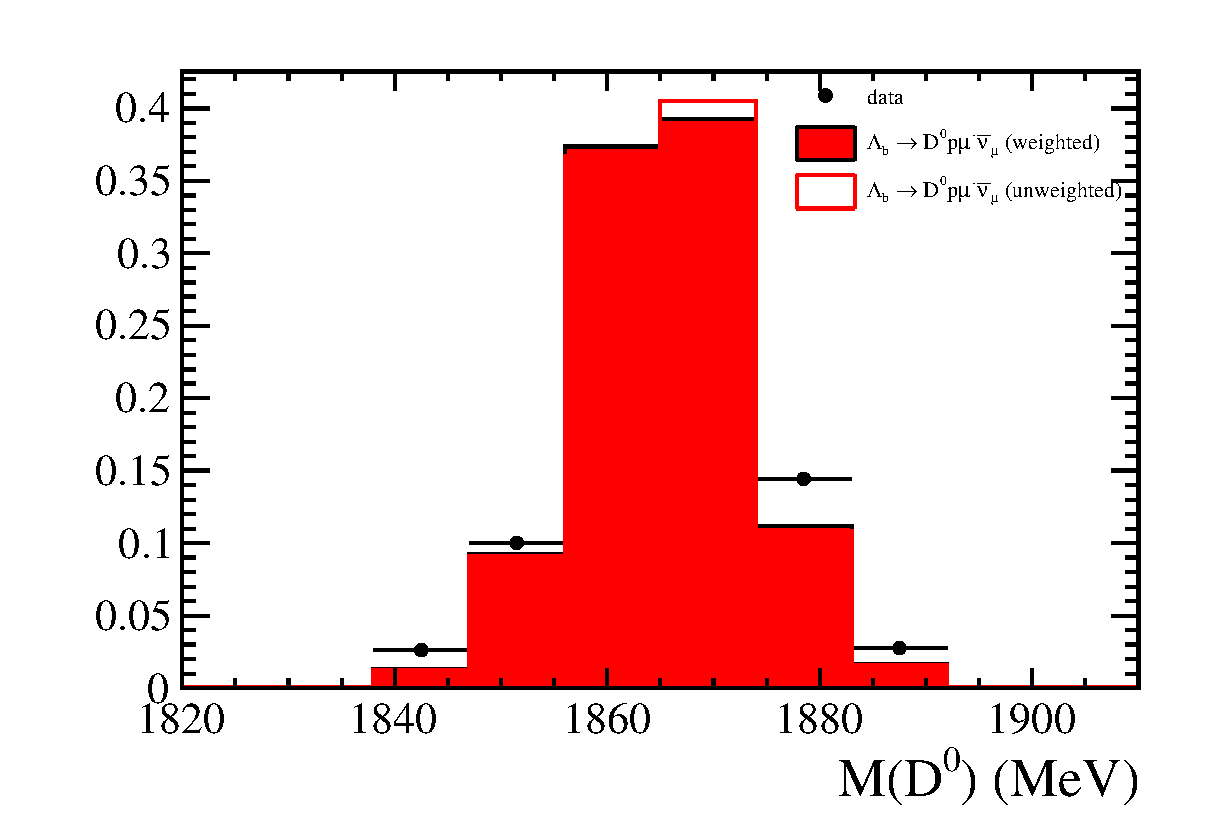
\includegraphics[width=0.8\textwidth]{LbToD0p/plots/data/D0_M}
	\caption{Invariant \Dz mass after the application of all selection requirements except for the \Dz mass itself.
             The arrows indicate where the selection requirements are applied.
             The colour-shaded areas shows the respective distributions for wrong sign (WS) combinations.
             A definition and explanation of wrong sign combinations is given at the end of section \ref{sec:Selection_D0pmu}}
	\label{fig:plot_mD0}
\end{figure}

\subsection{Reconstruction of the \Dz\mun candidate}
\label{sec:Selection_D0mu}
Having reconstructed the \Dz candidate one needs a muon track to combine them.
The motivation for the requirements on the muon track is analagous to the kaon and pion for the \Dz reconstruction.
Thus they will be just briefly mentioned:
The muon is required to have a minimum transverse momentum of 1.2\gev and a minimum momentum of 6\gev.
The track \chisqndf is smaller than 4 and the \chisqip with respect to the primary vertex larger than 9.
PIDmu is required to be greater than 0.3.
It might happen, that several hits in the detector are incidentally combined to a track albeit coming from different tracks.
The so called ghost probablity gives a measure of this issue and is required to be less than 0.5 for the muon track.

For the combination of \Dz and \mun the vertex shall be again of good qualitiy, i.e. \chisqvtx/ndf $<3$.
To avoid completely random combinations the invariant \Dz\mun mass is required to be between 2.2 and 8.0 \gev and a minimum transverse momentum of 3 \gev.
The minimum DIRA of the \Dz\mun candidate is 0.999.
With a requirement on the flight distance \chisq to be greater than 25 it is ensured that the \Dz\mun decay vertex is certainly displaced form the primary vertex.

\subsection{Reconstruction of the \Lb (\Dz\mun\proton) candidate}
\label{sec:Selection_D0pmu}
The proton's momentum and transverse momentum is required to be larger than 15 \gev and 1 \gev respectively for a good particle identification and to exclude protons boosted from the primary interaction.
To reduce the amount of fake protons, i.e. pions or kaon that are misidentified as protons, tight particle idenitification requirements are applied: PIDp $> 10$ and PIDp$-$PIDK $> 10$.
Having the definition of the PIDx variable in equation \ref{eq:PIDdef} in mind, PIDx serves always as distinction between a particle $x$ and a pion.
Thus, the difference between PIDp and PIDK enables for a better distinction between protons and kaons, since
\begin{align*}
    \text{PIDp}-\text{PIDK} &= \left(\ln \mathcal{L}_{\proton} - \ln \mathcal{L}_\pion\right) - \left(\ln \mathcal{L}_{\kaon} - \ln \mathcal{L}_\pion\right) \\
    & = \left(\ln \mathcal{L}_{\proton} - \ln \mathcal{L}_{\kaon}\right).
\end{align*}
The \chisqip with respect to the primary vertex is greater than 25, since the proton must not come from the primary vertex.
In contrast, the proton should make a good vertex with the \Dz\mun candidate.
It is thus required that the \logIP of the proton with respect to the \Dz\mun vertex is smaller than 1.
It should be noted, that throughout this thesis, the simple label \logIP refers to this variable.
This last requirement on \logIP is not applied in the signal fit to distinguish nonresonant signal and background as will be thoroughly explained in chapter \ref{sec:Signalfit}.

For the combined \Dz\mun\proton candidate the requirement on the angle $\alpha$ between flight direction and momentum is the tightest compared to the daughter candidates.
This is obvious since the impact of the detector resolution leading to a discrepancy between flight direction and momentum should be the smallest for the first decay of the decay chain.
An angle $\alpha < 0.015$ is required, which is equivalent to a DIRA $\gtrsim 0.999999$.

As stated at the beginning of this chapter, the information on the neutrino is missing in the reconstruction.
Thus, the reconstructed \Lb mass is smeared out and does not peak at the nominal \Lb mass of 5619.5\mev.
However, there are different ways to at least partially account for the missing neutrino.
One of them is the so called \textsc{corrected mass} of the \Lb.
It is defined as
\begin{align}
    m_{\text{corr}} = \sqrt{m_{\Dz\mun\proton}^2 + p_{\perp}^2} + p_{\perp}, \label{eq:correctedMass}
\end{align}
where $m_{\Dz\mun\proton}$ denotes the invariant mass of the \Dz\mun\proton candidate and $p_\perp$ its transverse momentum perpendicular to the \Lb flight direction, which is measured by the connection of the primary vertex and the \Lb decay vertex \cite{CorrectedMass}.
It is the minimum correction to the \Lb candidate if any daughters are missing.
If only a massless particle is missed the corrected mass would be the mass of the \Lb \cite{HLT2_Topological}.
This can be seen as follows:
In the rest frame of the \Lb, the \Lb mass can be written as
\begin{align}
    m_{\Lb} &= E_{\text{vis}} + E_{\text{miss}} \\
            &= \sqrt{M_{\text{vis}}^2 + p_{\perp, \text{vis}}^2 + p_{\parallel, \text{vis}}^2} + \sqrt{M_{\text{miss}}^2 + p_{\perp, \text{miss}}^2 + p_{\parallel, \text{miss}}^2},
\end{align}
where the index vis denotes the respective quantities of the visible, i.e. reconstructed particles and miss the ones of the missing particles.
If the missing particle is massless and if one changes to the \Lb rest frame, where $p_{\perp, \text{vis}} = p_{\perp, \text{miss}} = p_\perp$ and $p_{\parallel, \text{vis}} = p_{\parallel, \text{miss}} = p_\perp$ the \Lb mass becomes
\begin{align}
    m_{\Lb} = \sqrt{M_{\text{vis}}^2 + p_{\perp}^2 + p_{\parallel}^2} + \sqrt{p_{\perp}^2 + p_{\parallel}^2}.
\end{align}
Furthermore, if the longitudinal momentum can be ignored in the present rest frame the \Lb mass is described by the corrected mass $m_\text{corr}$ \cite{bQuark_LEP, Kodama:1991ij}.
Hence, it is required that the corrected \Lb mass lies around its PDG mass $M(\Lb)=(5619.5 \pm 0.4)\mev$ \cite{PDG} between 5 and 6 \gev.
Figure \ref{fig:plot_correctedMass} shows the distribution of the corrected \Lb mass.
Due to the correction of the missing neutrino it peaks near the PDG mass as explained above.
\begin{figure}[tb]
	\centering
	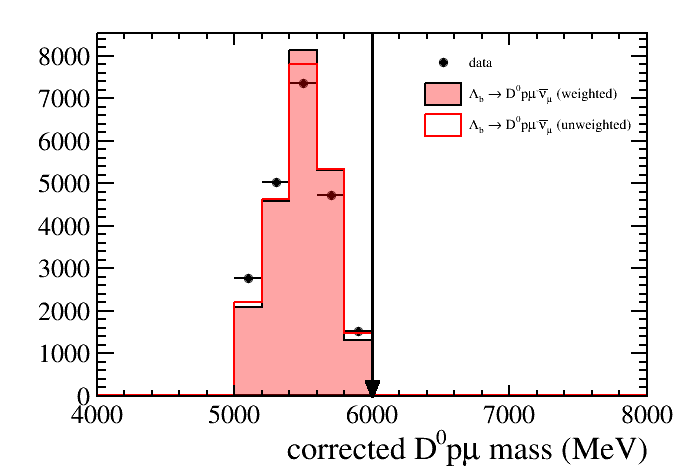
\includegraphics[width=0.8\textwidth]{LbToD0p/plots/data/Bh_BPVCORRM}
	\caption{Corrected \Lb mass after the application of all selection requirements except for the corrected \Lb mass itself.
             The arrows indicate where the selection requirements are applied.
             The colour-shaded areas shows the respective distributions for wrong sign (WS) combinations.
             The corrected \Lb mass tends to peak near the nominal \Lb mass of $M(\Lb)=(5619.5 \pm 0.4)\mev$ \cite{PDG}.}
	\label{fig:plot_correctedMass}
\end{figure}

Another background might be the decay \decay{\Lb}{\Dz\proton\pim}, where the pion is misidentified as muon.
In this case, all final state particles are reconstructed and the invariant \Dz\mun\proton mass peaks around the \Lb mass.
To veto such backgrounds only events with an invariant \Dz\mun\proton mass of less than 5.5 \gev are selected.
A detailed discussion of these backgrounds can be found in chapter \ref{sec:Backgrounds}, especially Figure \ref{fig:plot_D0pmuMass} visualises this veto.

\begin{table}[tb]
    \centering
    \caption{Summary of the selection requirements for the decay \LbToDpmunuX.}
    \label{tab:cuts_D0p}
    \begin{tabular}{r|ll}
        \hline
                & Variable            & Value           \\
        \hline
        Event   
        & number of long tracks       & $< 250$         \\
        \hline
        \mun 
        & Momentum                    & $> 6 \gev$      \\
        & Transverse momentum         & $> 1.2 \gev$    \\
        & Ghost probability           & $< 0.5$         \\
        & Track \chisq/ndf            & $< 4$           \\
        & \chisqip w.r.t. PV          & $> 9.0$         \\
        & PIDmu                       & $> 0.3$         \\
        \hline
        $D^0 \to K^-\pi^+$
        & Daughter momentum           & $> 2 \gev$      \\
        & Daughter transverse momentum& $> 300.0 \mev$  \\
        & Daughter ghost probablity   & $< 0.5$         \\
        & Daughter track \chisq/ndf   & $< 4$           \\
        & Daughter \chisqip w.r.t. PV & $> 4$           \\
        & \Km daughter PIDK           & $> 4$           \\
        & \pip daughter PIDK          & $< 10$          \\
        & \chisqvtx/ndf               & $< 6$           \\
        & DIRA w.r.t. PV              & $> 0.99$        \\
        & Mass difference to PDG      & $< 25 \mev$     \\
        & Flight distance w.r.t. PV   & $> 5 \mm$       \\
        \hline
        $D^0\mun$
        & Mass                            & $\in \left[2.2, 8.0\right] \gev$ \\
        & \chisqvtx/ndf                   & $< 3$                            \\
        & DIRA w.r.t. PV                  & $> 0.999$                        \\
        & Flight distance \chisq w.r.t. PV& $ > 25 $                         \\
        & Transverse momentum             & $ > 3000 \mev $                  \\
        \hline
        \proton
        & \chisqip w.r.t. PV              & $ > 25 $    \\
        & PIDp$-$PIDK                     & $ > 10 $    \\
        & PIDp                            & $ > 10 $    \\
        & Momentum                        & $ > 15\gev$ \\
        & Transverse momentum             & $ > 1 \gev$ \\
        & \logIP w.r.t. \Dz\mun vertex    & $ < 1 $     \\
        \hline
        $D^0\mun\proton$
        & $\arccos$(DIRA) w.r.t. PV       & $ < 0.015 $                   \\
        & Mass                            & $ < 5.5 \gev $                \\
        & Corrected mass                  & $ \in \left[5, 6\right] \gev $\\ 
        \hline
    \end{tabular}
\end{table}

Table \ref{tab:cuts_D0p} summarises all selection requirements mentioned in the last sections.
After the reconstruction and application of these requirements there are in total 21444 \LbToDpmunuX candidates left for the analysis.
In the nominal signalfit the cut on \logIP is not applied.
In this case, there are 34760 candidates available.
Figure \ref{fig:plot_mD0p_logIP} shows the invariant \Dz\proton mass (top) and the \logIP distribution (bottom). 
The first one is used for a spectroscopical analysis later.
If this thesis refers to the \Dz\proton mass, there is rather the quantity $\MDp - M(\Dz) + M_\text{PDG}(\Dz)$, where one first subtracts the reconstructed \Dz mass and then adds up the nominal \Dz mass from the PDG.
With this trick, one ``subtracts" the finite width from the \Dz\proton mass spectrum and improves the mass resolution.
\begin{figure}[tb]
	\centering
	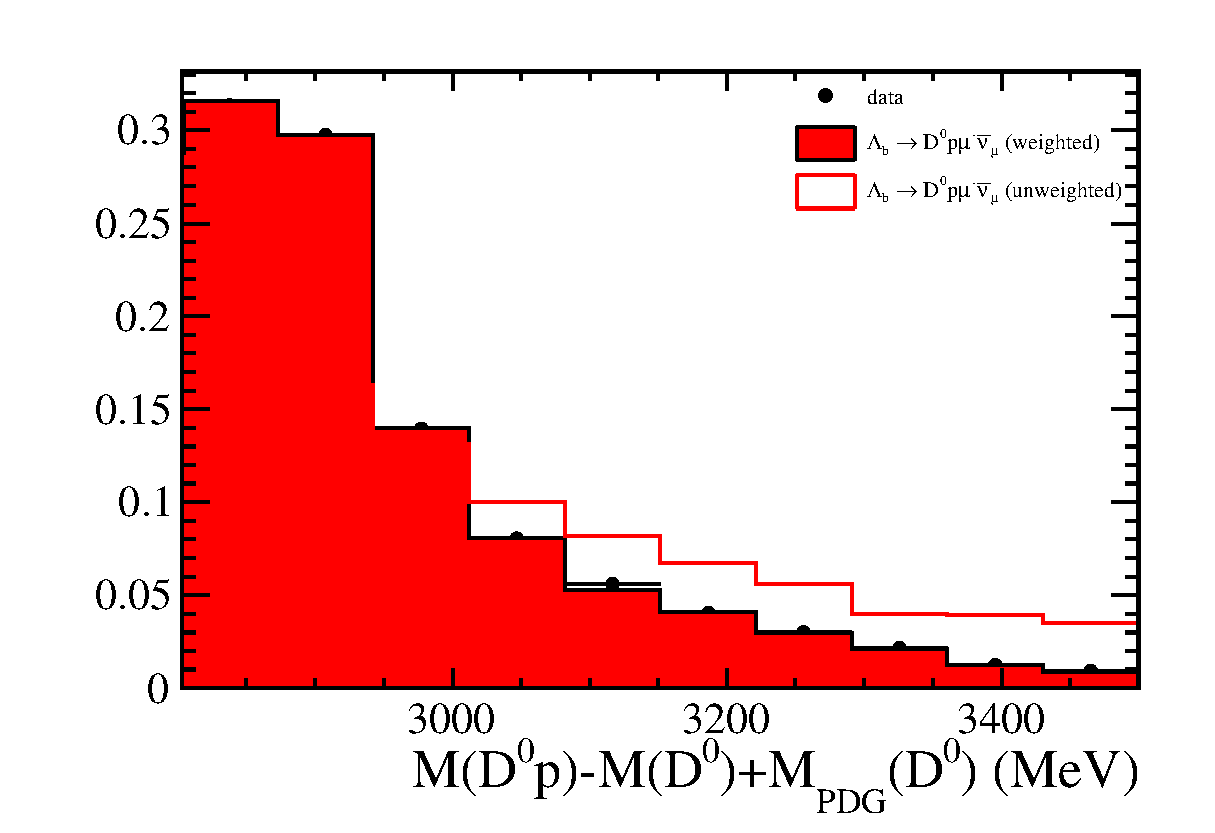
\includegraphics[width=\textwidth]{LbToD0p/plots/data/Bh_DELTA_MASS} \\
	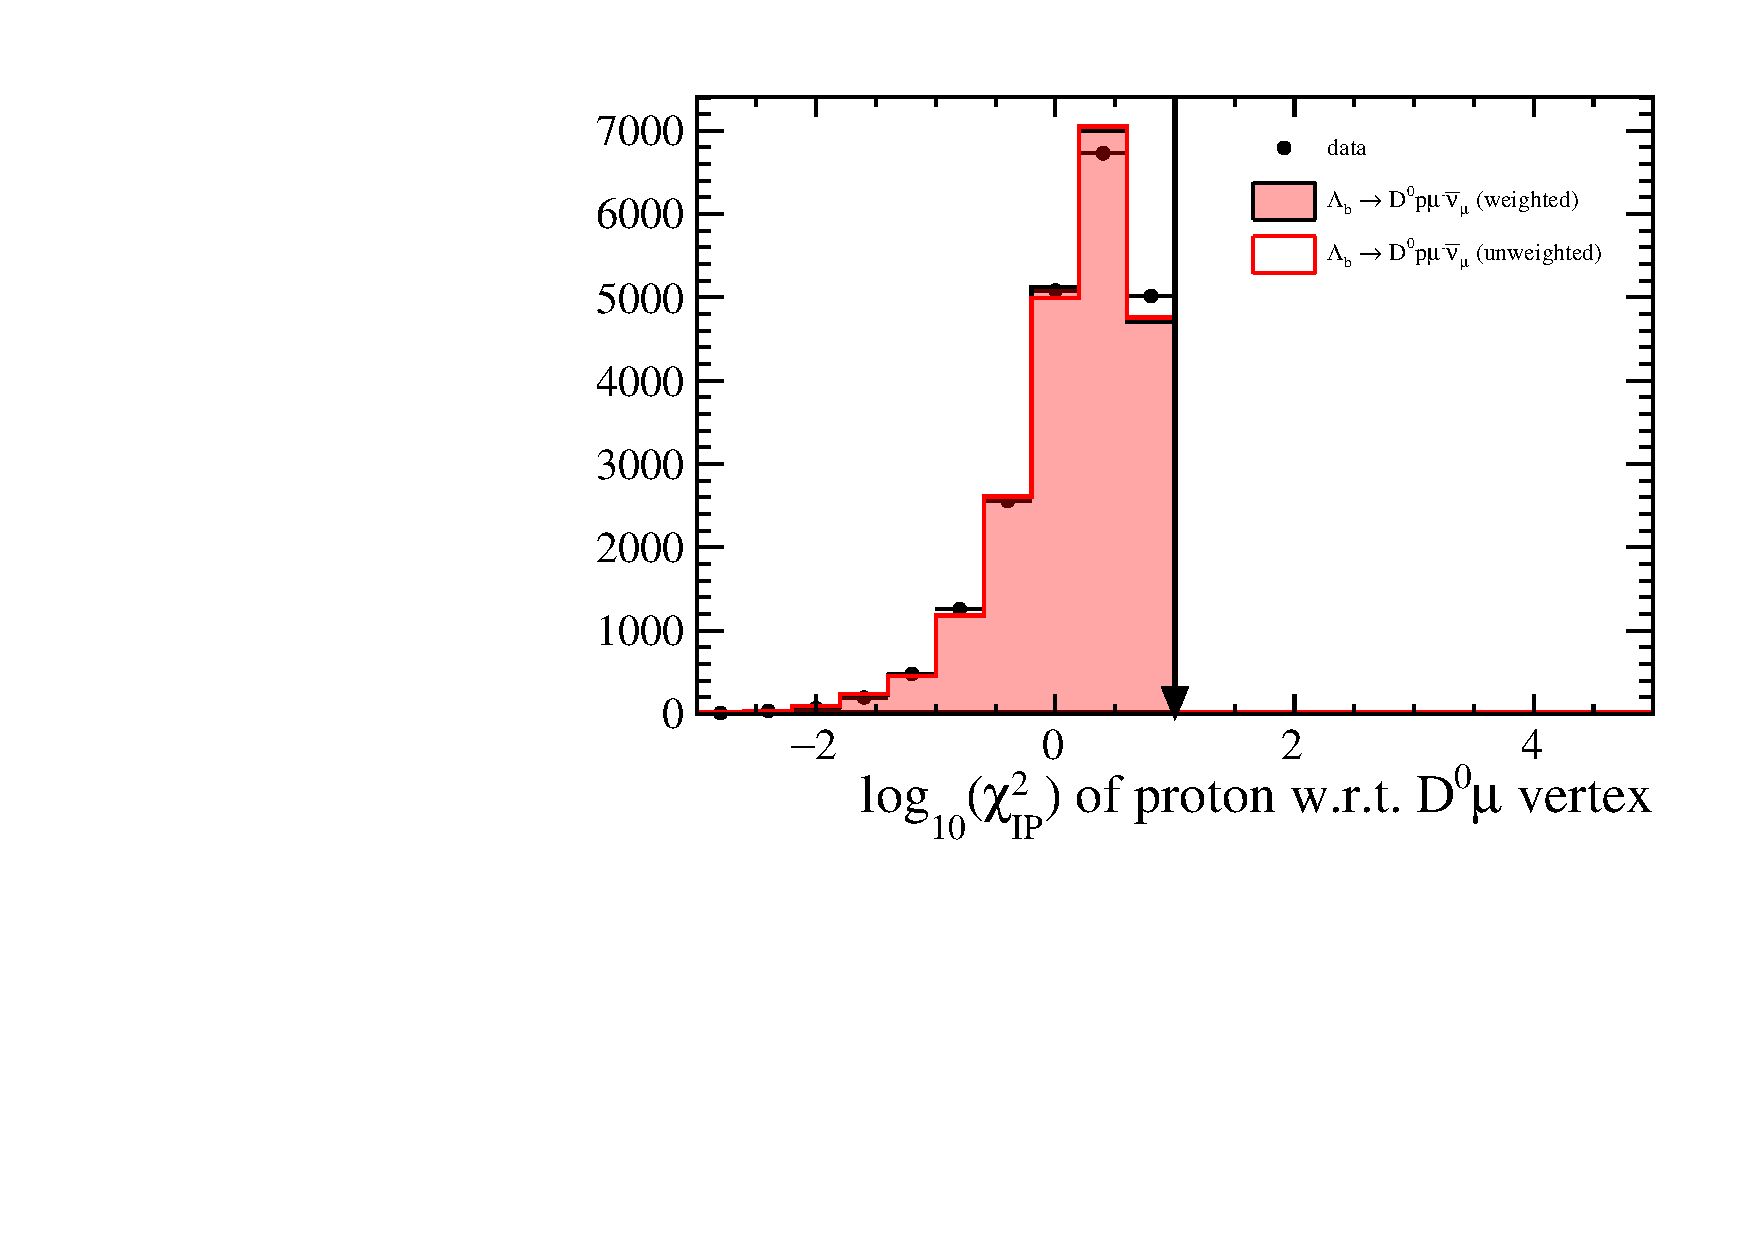
\includegraphics[width=\textwidth]{LbToD0p/plots/data/logIP}
	\caption{Invariant \Dz\proton mass (top) after the application of all selection requirements and \logIP distribution (bottom) after all requirements except for \logIP itself.
             The arrow in the \logIP distribution indicates where the selection requirement is applied.
             The colour-shaded areas shows the respective distributions for wrong sign (WS) combinations.}
	\label{fig:plot_mD0p_logIP}
\end{figure}
Some peaking structures can be seen in the spectrum, indicating that the decay \LbToDpmunuX might happen via intermediate resonances.
There is furthermore a broad distribution under the peaks.
This is assumed to be either background or nonresonant signal.
For their distinction, the \logIP distribution is used.
The plot confirms the explanation above:
Background events tend to peak at higher \logIP than signal events. 
This is justified by the so called \textsc{wrong sign (WS)} combinations.
To the physical decay \LbToDpmunuX there are also samples produced with one charge conjugated daughter particle.
There are three possibilities of combining a wrong sign particle:
\begin{itemize}
    \item \textbf{WSp:} \Dz\antiproton\mun final state
    \item \textbf{WSD0:} \Dzb\proton\mun final state
    \item \textbf{WSmu:} \Dz\proton\mup final state
\end{itemize}
There is not any physical process that allows the decay of a \Lb to these final states.
The most apparent violation of a physical law in these decays is the charge conservation.
Whereas the \Lb is electrically neutral, the final states of WSp and WSmu have a total charge of $\mp 2$.
For the WSD0 combinations, the electrical charge is fine, but the decay \decay{\Lb}{\Dzb\proton\mun} would require the quark transition \bquark \to \cquarkbar, which is forbidden in the Standard Model.
Thus if one reconstructs such unphysical decays these either arise due to random combinations of particle tracks or due to true physical decays, where one misidentifies a particle.
As example for the latter case serves a decay like \decay{\Bz}{\Dz\mun\pip\pip\piz} where one misidentifies the \piz as \antiproton and misses the two \pip.
Being caused by either random combinations or misidentification of particles, the wrong sign events provide first, rough estimate of the \LbToDpmunuX background behaviour.

\section{Reconstruction of the decay \LbToLcmunu}
The reconstruction of the \LbToLcmunu channel with \LcTopKpi is done quite similarly to the decay \LbToDpmunuX.
The main difference between those two channels is, that the proton is now combined with the \Km\pip to make a \LcTopKpi instead of being comined with the \Dz\mun.
As to the rest, the topology is analogous to \LbToDpmunuX.
The lifetime of the \Lb is long enough, such that the \Lb decays at a secondary vertex into a \Lc and \mun.
Like the \Dz, the \Lc flies another distance, finally decaying at a tertiary vertex into \pKpi.
The strategy for the selection is thus to find decays with the signature $X_{b} \rightarrow (\Lambda_c^+ \rightarrow K^- \pi^+ p^+) \mu^- \bar{\nu}_{\mu} X$.

\subsection{Reconstruction of the \Lc (\pKpi) candidate}
First of all, requirements on the tracks of the final state particles \proton, \kaon and \pion are made.
These are required to have a minimum momentum of 2\gev and a transverse momentum of 250\mev, their ghost probability should be less than 0.5 and the \chisqip with respect to the primary vertex is greater than 4.
The motivation for these cuts are the same as for the \Dz reconstruction in Section \ref{sec:Selection_D0}:
a good vertex quality, tracks not pointing to the primary vertex, good kinematics for particle identification and for not being bent out by the magnet.
To be compatible to the \LbToDpmunuX decay and to ensure a similar reconstruction of the proton, the requirements on the proton are adopted from the \LbToDpmunuX reconstruction:
A minimum momentum of 15 \gev, a minimum transverse momentum of 1 \gev and a minimum \chisqip with respect to the primary vertex of 25 is required.
Furthermore fake protons are suppressed by demanding PIDp $> 10$ and PIDp$-$PIDK $> 10$.
The kaon must satisfy PIDK $>-5$ and the pion PIDK $< 20$.

For the combined \pKpi, i.e. \Lc candidate the vertex must be of good quality, guaranteed by \chisqvtx/ndf $< 3$.
Its DIRA is required to be larger than 0.99 to match flight direction and momentum.
The difference of the \Lc mass to its PDG value is required to be smaller than 80\mev only, since the \Lc sidebands are later used to subtract combinatorial backgrounds below the \Lc mass peak.
Aside from a minimum transverse momentum of 2.1 \gev, \textsc{prompt} \Lc, i.e. \Lc directly coming from the primvary vertex, are supressed by requiring the logarithm of the \Lc impact parameter to be grater than -1.5 and a flight distance \chisq of more than 25, both with respect to the primary vertex.
Figure \ref{fig:plot_Lc_M} shows a clear peak of the invariant \Lc mass.
\begin{figure}[tb]
    \centering
	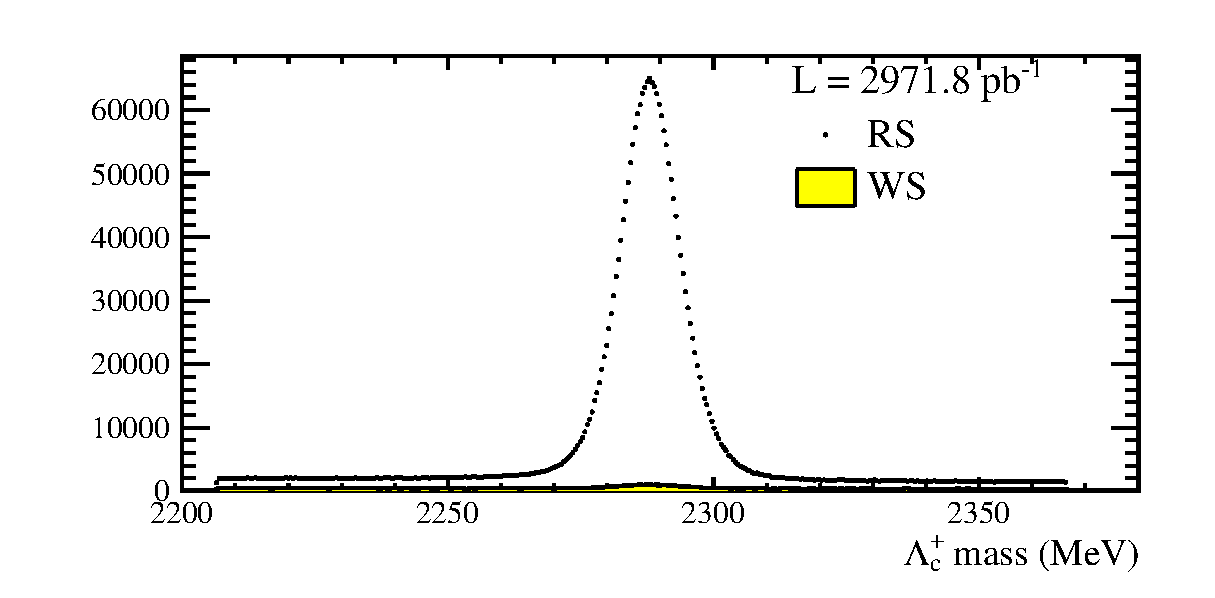
\includegraphics[width=\textwidth]{LbToLc/plots/data/Lc_M}	
	\caption{Plot of the invariant \pKpi mass distribution. A clear mass peak identified as the \Lc can be seen. The yellow shaded area shows events with the WS combination \Lc\mup.}
	\label{fig:plot_Lc_M}
\end{figure}

\subsection{Reconstruction of the \Lb (\Lc\mun) candidate}
The reconstruction of the muon track is completely analogous to the description in Section \ref{sec:Selection_D0mu} and hence not discussed here again.
The combined \Lc\mun, i.e. the \Lb candidate should make a good vertex with a maximum \chisqvtx of 6.
Its DIRA is required to be larger than 0.999.
Being a semileptonic decay again, only a loose selection on the invariant \Lc\mun mass can be applied.
It must have a mass between 2.2 and 8.0 \gev.

Compared to \LbToDpmunuX, main backgrounds are not assumed to be of combinatorial nature, but rather \Lb decays into excited \Lc states.
A good example is the decay \decay{\Lb}{\LcRes{(2595)}\mun\neumb} with \decay{\LcRes{(2595)}}{\Lc\piz}, where the \piz is not reconstructed.
Its decay topology does not differ from \LbToLcmunu, because the \LcRes{(2595)} decays immediately.
However, if the massive \piz is missing in addtion, the the corrected \Lb mass should be shifted to lower masses compared to \LbToLcmunu.
That is why there is not any requirement made on the \Lb corrected mass here.
The different behaviour of the corrected masses is used in the normalisation fit in Chapter \ref{sec:Normalisationfit}  to disentangle the signal from those backgrounds.
\begin{table}[tb]
    \centering
    \caption{Summary of the selection requirements for the reconstruction of \LbToLcmunu candidates.}
    \label{tab:cuts_Lc}
    \begin{tabular}{r|ll}
        \hline
                & Variable          & Value \\
        \hline
        Event   & number of long tracks       & $< 250$ \\
        \hline
        \mun
        & Transverse momentum         & $> 1 \gev$  \\
        & Momentum                    & $> 6 \gev$  \\
        & Ghost probability           & $< 0.5$     \\
        & Track \chisq/ndf            & $< 4$       \\
        & \chisqip w.r.t. PV          & $> 9.0$     \\
        & PIDmu                       & $> 0.3$     \\
        \hline
        \LcTopKpi
        & Daughter momentum           & $> 2 \gev$    \\
        & Daughter transverse momentum& $> 250.0 \mev$\\
        & Daughter ghost probability  & $< 0.5$       \\
        & Daughter \chisqip w.r.t. PV & $> 4.0$       \\
        & \proton daughter PIDp       & $> 10$ \\
        & \proton daughter PIDp$-$PIDK& $> 10$ \\
        & \proton daughter \ptot      & $> 15 \gev$ \\
        & \proton daughter \pt        & $> 1 \gev$ \\
        & \proton daughter \chisqip w.r.t. PV & $> 25 $    \\
        & \Km daughter PIDK           & $> -5.0$     \\
        & \pip daughter PIDK          & $< 20.0$     \\
        & \chisqvtx/ndf               & $< 3$ \\
        & DIRA w.r.t. PV              & $> 0.99$     \\
        & Mass diff. to PDG           & $< 80 \mev$  \\
        & Transverse momentum         & $>2.1 \gev$  \\
        & $\log_{10}$(IP) w.r.t. PV   & $ > - 1.5 $ \\
        & Flight distance \chisq w.r.t. PV  & $> 25$ \\
        \hline
        \Lc\mun
        & Mass                            & $\in \left[2.2, 8.0\right] \gev$ \\
        & \chisqvtx/ndf                   & $< 6$                            \\
        & DIRA w.r.t. PV                  & $> 0.999$                        \\
        \hline
    \end{tabular}
\end{table}

Table \ref{tab:cuts_Lc} summarises all requirements for the reconstruction of the \LbToLcmunu candidates.
After application of all these requirements there are in total 2670999 \LbToLcmunu candidates left for the further analysis. 
Figure \ref{fig:plot_Lb_M_Lc} shows on the left-hand side the invariant mass distribution of the \Lb candidates and on the right-hand side the corrected \Lb mass distribution.
Whereas the \Lb mass is shifted to lower masses due to the missing neutrino, the corrected mass peaks close to the PDG mass of about 5619.5\mev \cite{PDG}.
\begin{figure}[tb]
    \centering
	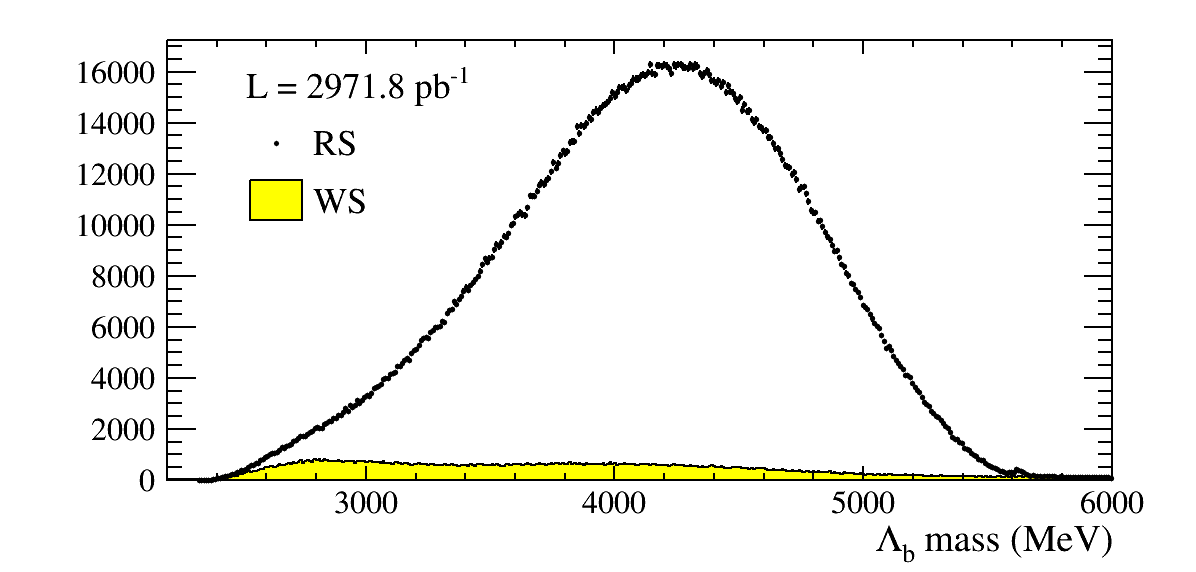
\includegraphics[width=0.49\textwidth]{LbToLc/plots/data/Lb_M} 	
	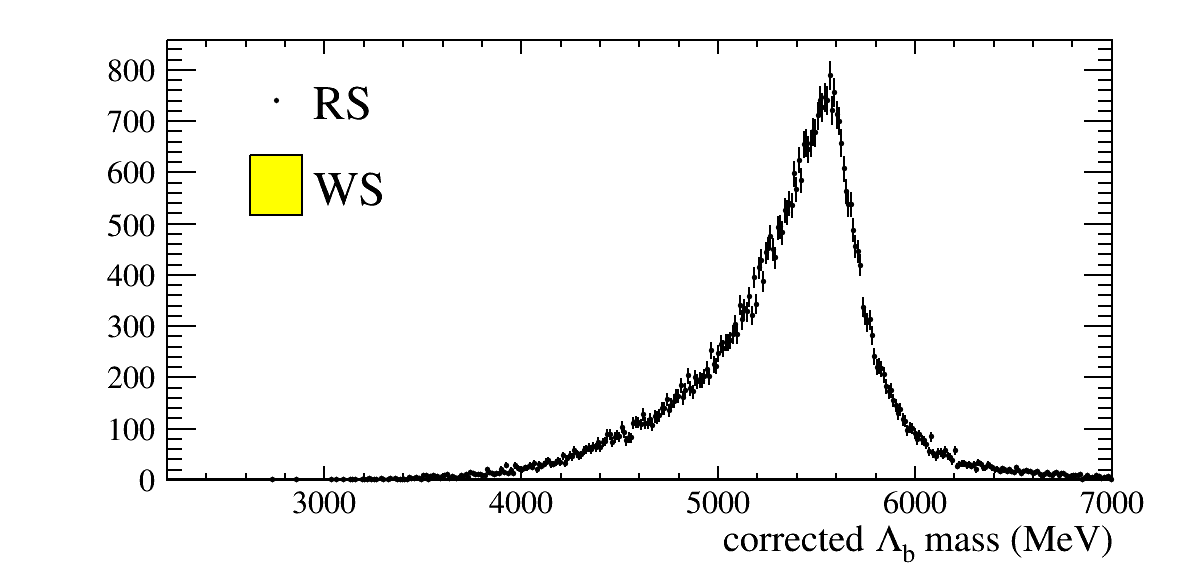
\includegraphics[width=0.49\textwidth]{LbToLc/plots/data/Lb_BPVCORRM}	
	\caption{Plot of the invariant \Lb mass distribution (left) and of the corrected \Lb mass (right). Due to the missing neutrino the \Lb mass peak is shifted to lower masses compared its nominal mass of 5619.5 \mev. With the correction for the missing neutrino, the peak is close to the nominal \Lb
    mass. The yellow shaded area shows events with the WS combination \Lc\mup.}
	\label{fig:plot_Lb_M_Lc}
\end{figure}
